\documentclass{standalone}
\usepackage{hsbcommon}
\begin{document}
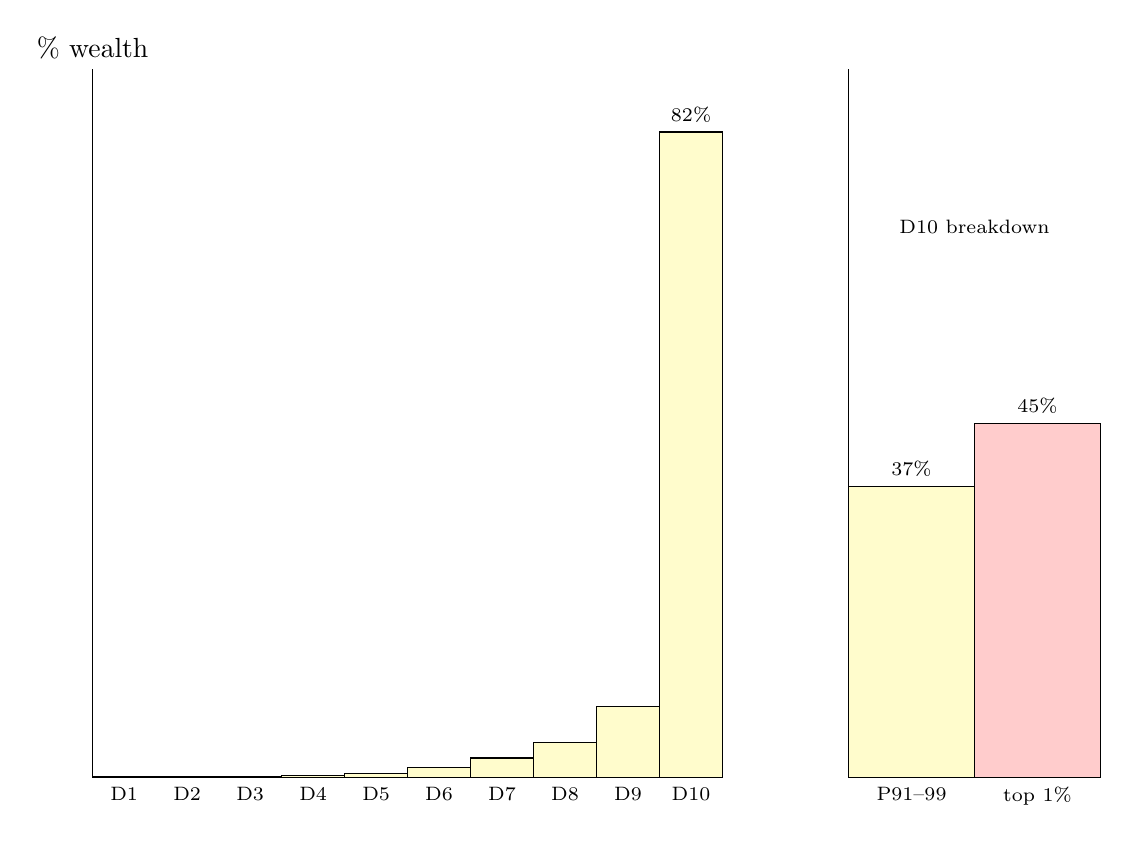
\begin{tikzpicture}[y=0.1cm,x=0.8cm]

    \tikzset{mystyle/.style={fill=yellow!20}}
    \tikzset{topstyle/.style={fill=red!20}}

    % Main decile chart
    \draw (0,0) -- (10,0);
    \draw (0,0) -- (0,90) node[above] {\% wealth};

    \foreach [count=\i] \ii in {%
        0.1, 0.15, 0.2, 0.25, 0.5,
        1.3, 2.5, 4.5, 9.0, 82.0%
    }{
    \draw[mystyle] (\i-1,0) rectangle (\i,\ii);
    \node[below] at (\i-0.5,0) {\scriptsize D\i};
    }
    \node[above] at (9.5,82) {\scriptsize 82\%};

    % Inset: zoom into D10 split (91-99th vs top 1%)
    \begin{scope}[shift={(12,0)}, y=0.1cm]
        \draw (0,0) -- (4,0);
        \node at (2,70)  {\scriptsize D10 breakdown};
        \draw (0,0) -- (0,90);
        \draw[mystyle] (0,0) rectangle (2,37);
        \node[below] at (1,0) {\scriptsize P91--99};
        \node[above] at (1,37) {\scriptsize 37\%};
        \draw[topstyle] (2,0) rectangle (4,45);
        \node[below] at (3,0) {\scriptsize top 1\%};
        \node[above] at (3,45) {\scriptsize 45\%};
    \end{scope}

\end{tikzpicture}
\end{document}